%% ----------------------------------------------------------------
%% Thesis.tex -- MAIN FILE (the one that you compile with LaTeX)
%% ---------------------------------------------------------------- 

% Set up the document
\documentclass[a4paper, 11pt, oneside]{Thesis}  % Use the "Thesis" style, based on the ECS Thesis style by Steve Gunn
\graphicspath{Figures/}  % Location of the graphics files (set up for graphics to be in PDF format)
% \usepackage{graphicx}
% Include any extra LaTeX packages required
\usepackage[square, numbers, comma, sort&compress]{natbib}  % Use the "Natbib" style for the references in the Bibliography
\usepackage{verbatim}  % Needed for the "comment" environment to make LaTeX comments
\usepackage{vector}  % Allows "\bvec{}" and "\buvec{}" for "blackboard" style bold vectors in maths
\usepackage{braket}
\usepackage{amsmath}
\usepackage{physics}
\usepackage{dsfont}
\usepackage{subcaption}
\usepackage{caption}

\hypersetup{urlcolor=blue, colorlinks=true}  % Colours hyperlinks in blue, but this can be distracting if there are many links.

%% ----------------------------------------------------------------
\begin{document}
\frontmatter      % Begin Roman style (i, ii, iii, iv...) page numbering

% Set up the Title Page
\title  {The Dance of Atoms}
\authors  {\texorpdfstring
            {\href{https://debasishpanda529.github.io}{Debasish Panda}}
            {Debasish Panda}
            }
\addresses  {\groupname\\\deptname\\\univname}  % Do not change this here, instead these must be set in the "Thesis.cls" file, please look through it instead
\date       {November 2024}
\subject    {}
\keywords   {}

\maketitle
%% ----------------------------------------------------------------

\setstretch{1.3}  % It is better to have smaller font and larger line spacing than the other way round
% Define the page headers using the FancyHdr package and set up for one-sided printing
\fancyhead{}  % Clears all page headers and footers
\rhead{\thepage}  % Sets the right side header to show the page number
\lhead{}  % Clears the left side page header

\pagestyle{fancy}  % Finally, use the "fancy" page style to implement the FancyHdr headers

%% ----------------------------------------------------------------
% The "Funny Quote Page"
\pagestyle{empty}  % No headers or footers for the following pages

\null\vfill
% Now comes the "Funny Quote", written in italics
\textit{``Nunc scio nihil.''}

\begin{flushright}
-- perhaps some disillusioned Roman philosopher in his 20's
\end{flushright}

\vfill\vfill\vfill\vfill\vfill\vfill\null
\clearpage  % Funny Quote page ended, start a new page
%% ----------------------------------------------------------------

% The Preface Page
\addtotoc{Preface}  % Add the "Preface" page entry to the Contents
\abstract{
\addtocontents{toc}{\vspace{1em}}  % Add a gap in the Contents, for aesthetics

Semiconductor-based devices have become the lifeblood of modern civilisation, powering the tiniest microprocessor to the largest of the ICBMs. In our quest for smaller and still smaller transistors, we have now hit a fundamental barrier beyond which deterministic Newtonian mechanics is helpless and quantum mechanics reigns with all its glory of probabilistic chaos. This calls immediately for a fundamental understanding of the quantum mechanical nature of such beyond-Moore devices, viz., \textit{quantum devices}. This article is devoted to a brief exploration of such concepts, starting from simple toy models of quantum condensed matter systems---reviewing the tight-binding ansatz, physics of quantum bands, second quantization---and touching upon the state-of-the-art in modern condensed matter---quantum topology and topological electronics. 

}

\clearpage  % Preface ended, start a new page
%% ----------------------------------------------------------------

\pagestyle{fancy}  %The page style headers have been "empty" all this time, now use the "fancy" headers as defined before to bring them back


%% ----------------------------------------------------------------
\lhead{\emph{Contents}}  % Set the left side page header to "Contents"
\tableofcontents  % Write out the Table of Contents

%% ----------------------------------------------------------------
\mainmatter	  % Begin normal, numeric (1,2,3...) page numbering

% only chapter name appears at the header instead of chapter number
\renewcommand{\chaptermark}[1]{\markboth{\thechapter.\ #1}{}}
\renewcommand{\chaptermark}[1]{\markboth{#1}{}}

\pagestyle{fancy}  % Return the page headers back to the "fancy" style

\fancyhead{}
\rhead{\thepage}
\lhead{\small\textit{\leftmark}}

% Include the chapters of the thesis, as separate files

\chapter{Second Quantisation}

Before we begin our incursion into the so-called 'second quantisation', we need to appreciate the reason why the need for second quantization arose. The properties of quantum condensed matter systems and, by extension, that of real materials are controlled by the \textit{collective behaviour} of electrons in the presence of some background potential due to an underlying crystal lattice. This statement, in fact, is a simpler rendition of the Bohr-Oppenheimer approximation. So, what factors do we need to consider during the analysis of a condensed matter system?
\begin{itemize}
    \item Focus on electrons and their collective dynamics
    \item Electrons are free to move from one orbital to another (tunnelling/hopping)
    \item They are subject to a background potential from the lattice
    \item They can interact with each other due to Coulomb repulsion
\end{itemize}
The question remains, how do we formulate the Hamiltonian for many-body systems? How do we encode anti-symmetry of fermions into this many-particle wavefunction? And most importantly, how do we find out the eigenstates/eigenvalues of momentum and/or energy of the system?  \par

So, how do we encode fermionic anti-symmetry in many-particle wavefunctions? \par

Consider a single-particle quantum state $\phi_{\nu}(\vec{r})$, where $\nu$ refers to labels for the quantum state. The basis for a two-particle system is then given by 

\begin{equation*}
    \psi(\vec{r_{1}}, \vec{r_{2}}) = \frac{1}{\sqrt{2}}[\phi_{\nu_{1}}(\vec{r_{1}}) \phi_{\nu_{2}}(\vec{r_{2}}) - \phi_{\nu_{1}}(\vec{r_{2}}) \phi_{\nu_{2}}(\vec{r_{1}})]
\end{equation*}

This basis satisfies the anti-symmetry property, and also, there happens to be a less verbose manner through which we can express such wavefunctions - Slater's determinants. \par

For a generalized $N$-particle system such that the basis states are perfectly anti-symmetric under exchanging the labels of any two particles, the wavefunction can be expressed as

\begin{equation*}
    \psi(\vec{r_{1}}, \vec{r_{2}},..., \vec{r_{N}}) = \frac{1}{\sqrt{N!}} \begin{bmatrix}
        \phi_{\nu_{1}}(\vec{r_{1}}) & \phi_{\nu_{2}}(\vec{r_{1}}) & ... & \phi_{\nu_{N}}(\vec{r_{1}}) \\
        \phi_{\nu_{1}}(\vec{r_{2}}) & \phi_{\nu_{2}}(\vec{r_{2}}) & ... & \phi_{\nu_{N}}(\vec{r_{2}}) \\
        . & . &  & . \\
        . & . &  & . \\
        . & . &  & . \\
        \phi_{\nu_{1}}(\vec{r_{N}}) & \phi_{\nu_{2}}(\vec{r_{N}}) & ... & \phi_{\nu_{N}}(\vec{r_{N}})
    \end{bmatrix}
\end{equation*}

The 'first quantisation' principle cannot be used to satisfactorily explain condensed matter systems since calculations become cumbersome and expensive as the number of particles in the system increases, and the representation requires the number of particles, $N$, to be fixed. As $N$ approaches the limit associated with statistical physics, $N$ is allowed to fluctuate as per the grand canonical ensemble. Second quantisation or occupation number formalism is the standard way in which many-particle QM is formulated. It is based on the algebra of ladder operators.

\begin{itemize}
    \item Second quantisation provides a compact way of representing the many-body space of excitations.
    \item Properties of operators are now encoded in a single set of commutation/anti-commutation relations rather than in some explicit Hilbert space representation. 
\end{itemize}

In essence, second quantisation formalism offers us a significant computational advantage and a more compact and efficient representation of the Hamiltonian when dealing with many-particle quantum systems. For example, consider a \textit{symmetrised} $N$-particle wavefunction of fermions ($\zeta = -1$) or bosons ($\zeta = +1$) expressed in the form 

\begin{equation}
    \ket{\lambda_{1}, \lambda_{2},\ldots \lambda_{N}} = \frac{1}{\sqrt{N! \prod_{\lambda=0}^{\infty}n_{\lambda}!}} \sum_{\mathcal{P}}\zeta^{\mathcal{P}} \ket{\psi_{\lambda_{\mathcal{P}1}}} \otimes \ket{\psi_{\lambda_{\mathcal{P}2}}} \ldots \otimes \ket{\psi_{\lambda_{\mathcal{P}N}}}
\end{equation}

where $n_{\lambda}$ is the total number of particles in state $\lambda$ (for fermions, Pauli exclusion principle dictates that $n_{\lambda} = 0,1$, i.e. $n_{\lambda}! = 1$). The summation runs over all $N!$ permutations of the quantum numbers $\lambda_{i}$, and $\mathcal{P}$ denotes the parity \footnote{Parity is defined as the number of transpositions of two elements which brings the permutation ($\mathcal{P}_1, \mathcal{P}_2,\ldots \mathcal{P}_{N}$)) back to the ordered sequence (1,2,\ldots N)}. \par

Second quantisation formalism provides for a much more condensed and intuitive representation for the generalised wavefunction via the \textbf{vacuum state} $\ket{\Omega}$, and a set of creation (annihilation) \textbf{field operators} $c_{\lambda}$ ($c_{\lambda}^{\dagger}$), as follows:

\begin{equation}
\label{eq:eq1}
    c_{\lambda} \ket{\Omega} = 0, \quad \frac{1}{\sqrt{\prod_{\lambda}n_{\lambda}!}} c_{\lambda_N}^{\dagger} \ldots c_{\lambda_1}^{\dagger} \ket{\Omega} = \ket{\lambda_{1}, \lambda_{2},\ldots \lambda_{N}}
\end{equation}

In terms of physical interpretation, the operator $c_{\lambda}^{\dagger}$ creates a particle in state $\lambda$ while the operator $c_{\lambda}$ annihilates it. The commutation relations between these operators are captured via Clifford algebra \footnote{$[\hat{A},\hat{B}]_{\zeta} = \hat{A}\hat{B}-\zeta \hat{B}\hat{A}$ is the commutator $\zeta = 1$ (anticommutator $\zeta = -1$) for bosons (fermions). As per convention, the notation [.,.] denotes the commutator while \{.,.\} the anticommutator.}:

\begin{equation}
    [c_{\lambda},c_{\mu}^{\dagger}]_{-\zeta} = \delta_{\lambda,\mu}, \quad [c_{\lambda},c_{\mu}]_{-\zeta} = [c_{\lambda}^{\dagger},c_{\mu}^{\dagger}]_{-\zeta} = 0
\end{equation}

The physical interpretation of \ref{eq:eq1} and the commutation relations of the field operators is no trivial matter -- these equations imply that for \textit{any N}, the $N$-body wavefunction can be generated by an application of a set of $N$-independent operators to a vacuum state. Similarly, the formal definition of the general many-body or \textbf{Fock space} can be given as the direct sum $\oplus_{N=0}^{\infty}\mathcal{F}_N$, where $\mathcal{F}_N$ is defined as the linear span of all $N$-particle states $\ket{\lambda_{1}, \lambda_{2},\ldots \lambda_{N}} = \frac{1}{\sqrt{\prod_{\lambda}n_{\lambda}!}} c_{\lambda_N}^{\dagger} \ldots c_{\lambda_1}^{\dagger} \ket{\Omega}$. Intuitively, the Fock-subspaces $\mathcal{F}_N$ are generated by repeated action of creation operators on the vacuum space $\mathcal{F}_0$, and application of creation/annihilation field operator on a wavefunction takes it from one Fock-subspace to another. \par 

Before proceeding further, we need to determine the basis transformation for the field operators, and the Fourier transform of the operators from the real space to $k$-space (otherwise known as the momentum space). These results will prove incredibly useful while analysing the Hamiltonians for interacting fermionic systems. \par

\clearpage

\subsection{Change of basis}

The identity operator, $\mathcal{I}$ can be resolved as $\mathcal{I} = \sum_{\lambda=0}^{\infty}\ket{\lambda}\bra{\lambda}$. Using the relations $\ket{\tilde{\lambda}} = \sum_{\lambda}\ket{\lambda}\braket{\lambda|\tilde{\lambda}}$, $\ket{\lambda} = a_{\lambda}^{\dagger}\ket{\Omega}$, and $\ket{\tilde{\lambda}} = a_{\tilde{\lambda}}^{\dagger} \ket{\Omega}$, the transformation law is given by:

\begin{equation}
    c_{\tilde{\lambda}}^{\dagger} = \sum_{\lambda} \langle \lambda|\tilde{\lambda} \rangle c_{\lambda}^{\dagger}, \quad c_{\tilde{\lambda}} = \sum_{\lambda} \langle \tilde{\lambda}|\lambda \rangle c_{\lambda}
\end{equation}

\subsection{Fourier transform of field operators}

The physical interpretation provided for the creation (annihilation) operators states that they can be thought of as creating (annihilating) a particle in a state $\lambda$. In particular, this can be thought of as creating (annihilating) a particle at a dimensional site $r$, or equivalently, with a momentum $k$. This distinction is important since it is subtly related to the Heisenberg Uncertainty Principle -- the first scenario implies that the position of the particle is known with a very high certainty, and therefore is delocalised in momentum space and vice-versa. The transformation from real space to $k$-space and vice-versa is captured via Fourier transform of the field operators.

\begin{equation}
    \hat{c}_{r}^{(\dagger)} = \frac{1}{\sqrt{N}}\sum_{k}e^{-(+)ikr} \hat{c}_{k}^{(\dagger)}, \quad \hat{c}_{k}^{(\dagger)} = \frac{1}{\sqrt{N}}\int_{r}e^{-(+)ikr} \hat{c}_{r}^{(\dagger)}
\end{equation}

If we are dealing with discrete lattice sites, the Fourier transform has to be modified accordingly

\begin{equation}
    \hat{c}_{r}^{(\dagger)} = \frac{1}{\sqrt{N}} \sum_{k}e^{-(+)ikar}c_{k}^{(\dagger)}
\end{equation}

and $k$ lies inside the first Brillouin zone, i.e. $k \in \left[-\frac{\pi}{a},\frac{\pi}{a}\right]$ and $a$ is the lattice constant.

\section{Representation of operators}

Single particle or one-body operators $\hat{\mathcal{O}_{1}}$ acting in a $N$-particle Hilbert space, $\mathcal{F}^{N}$, generally take the form $\hat{\mathcal{O}_{1}} = \sum_{n = 1}^{N}\hat{o}_{n}$, where $\hat{o}_{n}$ is an ordinary single-particle operator acting on the $n$-th particle. A typical example is the kinetic energy operator $\hat{T} = \sum_{n}\frac{\hat{p}_{n}^{2}}{2m}$, where $\hat{p}_{n}$ is the momentum operator acting on the $n$-th particle. Since we have seen that, by applying field operators to the vacuum space, we can generate the Fock space in general and any $N$-particle Hilbert space in particular, it must be possible to represent any operator $\hat{\mathcal{O}_{1}}$ using the set of creation/annihilation operators. Here, we present the formal representation of a one-body operator using second quantization principles,

\begin{equation}
    \hat{\mathcal{O}_{1}} = \sum_{\lambda \mu \nu}\langle \mu | \lambda \rangle o_{\lambda}\langle \lambda | \nu \rangle \hat{c}^{\dagger}_{\mu} \hat{c}_{\nu} = \sum_{\mu \nu}\langle \mu|\hat{o}|\nu \rangle \hat{c}^{\dagger}_{\mu} \hat{c}_{\nu}
\end{equation}

Formally, the one-body operator, $\hat{\mathcal{O}_{1}}$, scatters a particle from a state $\nu$ into a state $\mu$ with probability amplitude $\braket{\mu|\hat{o}|\nu}$. \\

Two-body operators $\hat{\mathcal{O}_{2}}$ are needed to describe \textit{pairwise interactions} between particles. Although pair-interaction potentials are straightforwardly included in classical many-body theories, their embedding into conventional many-body quantum mechanics is made awkward by particle indistinguishability. Here again, we present the formal representation of a two-body operator using second quantization principles without providing a detailed derivation for the same.

\begin{equation}
    \hat{\mathcal{O}_{2}} = \sum_{\lambda \lambda^{\prime} \mu \mu^{\prime}} \langle \mu, \mu^{\prime}|\mathcal{O}_{2}|\lambda, \lambda^{\prime}\rangle \hat{c}_{\mu^{\prime}}^{\dagger} \hat{c}_{\mu}^{\dagger} \hat{c}_{\lambda} \hat{c}_{\lambda^{\prime}}
\end{equation}


\section{Tight Binding Models}

The beautiful simplicity embodied within the second quantisation formalism culminates with the ease with which it can be used to describe a many-particle system. Consider, for example, the free electron gas, with electrons occupying quantum states $\ket{k} = \ket{n_{k}}$, whose Hamiltonian can be expressed as

\begin{equation}
    \hat{H} = \sum_{k}\epsilon_{k}\hat{c}_{k}^{\dagger}\hat{c}_{k} = \sum_{k}\epsilon_{k}\hat{n}_{k}
\end{equation}

where $\epsilon_{k}$ represents the single-particle state of energy corresponding to the potential energy associated with orbital $\ket{k}$, and $\hat{n}_{k}$ represents the number operator. \par

Now, we shall introduce an additional layer of complexity to the problem by accounting for the interaction between fermionic particles constituting the system.

\begin{equation}
    \hat{H} = \sum_{i}\epsilon_{i} \: \hat{c}_{i}^{\dagger} \hat{c}_{i} + \sum_{i \neq j}t_{ij} \: \hat{c}_{i}^{\dagger} \hat{c}_{j}
\end{equation}

where $t_{ij}$ is the tunnelling matrix element corresponding to the tunnelling/hopping of an electron from orbital $\ket{i}$ to orbital $\ket{j}$, such that $\langle i|\hat{H}|j \rangle = t_{ij}$. Additionally, since the Hamiltonian is intrinsically Hermitian, it places a restriction on the elements of the tunnelling matrix, namely, $t_{ij} = t_{ji}^{*}$. Such tight-binding models can be used as a compact, and highly intuitive description of many-particle systems in terms of creation (annihilation) field operators. \par

Benzene provides an excellent toy model to illustrate the application of these principles to formulate its equivalent tight-binding Hamiltonian. The $p_{z}$ orbitals in benzene interact with only their nearest neighbors, which greatly simplifies the hopping terms associated with its $\pi$-bonded electronic network. 

\begin{equation*}
    \hat{H}_{\pi} = \epsilon \sum_{i=1}^{6} \hat{c}_{i}^{\dagger} \hat{c}_{i} + t \sum_{i=1}^{6} (\hat{c}_{i}^{\dagger} \hat{c}_{i+1} + \hat{c}_{i+1}^{\dagger} \hat{c}_{i})
\end{equation*}

\vspace{1cm}

\begin{figure}[h]
\centering
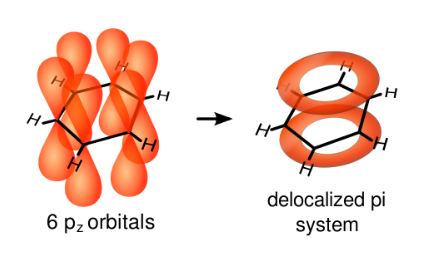
\includegraphics[scale=0.7]{benzene.png}
\caption{\textit{The $p_{z}$ orbitals of the respective carbon atoms in benzene interact with their nearest neighbours, forming a delocalized network of $\pi$-electrons}}\label{benzene}
\end{figure} % Second Quantisation

\chapter{Bandstructure}


\section{LCAO Theory}
Before presenting the more elegant manner in which electronic bandstructure of many-particle systems can be determined via a combination of the principles behind second quantisation formalism and Bloch's theorem, I would like to present the generic (or more bluntly, $obsolete$) technique of analysing bandstructure using the principles of first quantisation. \\

Consider a linear chain of identical hydrogenic atoms ($ns$ orbitals) with individual lattice points separated by a distance $a$. From the LCAO theory, the generalized wavefunction of the system can be expressed as a linear combination of orbitals at the lattice sites:
\begin{equation*}
    \psi = c_{1}\phi_{1} + c_{2}\phi_{2} + c_{3}\phi_{3} + ... = \sum_{n}c_{n}\phi_{n}
\end{equation*}

where $x_{n}$ is the position of the $n$th atom. The atoms, being identical, contribute equally to the LCAO in terms of their wavefunction amplitude but with different phase factors to account for their periodic distribution. More formally, this idea is captured via Bloch's theorem, which presents a generalised wavefunction for particles in a periodic lattice:
\begin{equation*}
    \psi_{k}(\vec{r}) = e^{i\vec{k}\cdot \vec{r}}u_{k}(\vec{r})
\end{equation*}

where $u_{k}(\vec{r})$ is called the \textit{cell function}, and represents atoms in the unit cell. For the toy model described above, the Bloch wavefunction is given by
\begin{equation}
    \psi_{k} = \sum_{n=1}^{N} e^{ikna}\phi_{n}
\end{equation}

The Bloch wavefunction incorporates the real-space symmetry of the lattice into the $k$-space in the sense that for $k > \frac{\pi}{a}$, the wavefunction merely acquires a global phase, and this does not affect the expectation value of measurables. The energy eigenvalue of the Bloch wavefunction serves as a direct measure of the $E-k$ relationship and is given by
\begin{equation}
    E = \frac{\int_{\mathcal{R}} \psi_{k}^{\dagger} \mathcal{H}\psi_{k}\: dx}{\int_{\mathcal{R}} \psi_{k}^{\dagger} \psi_{k}\: dx}
\end{equation}

The expectation value of the Hamiltonian can be simplified as
\begin{equation*}
    \int_{\mathcal{R}} \psi_{k}^{\dagger}\mathcal{H}\psi_{k} \: dx = \sum_{n=1}^{N} \sum_{m=1}^{N}e^{i(n-m)ka} \int_{\mathcal{R}} \phi_{m}^{\dagger}\mathcal{H}\phi_{n} \: dx
\end{equation*}

Applying the constraints of the tight-binding approximation, the integral term involved in RHS can be simplified into three distinct cases: $\alpha$ if $m = n$, i.e., the potential energy corresponding to each lattice site, $\beta$ if $|m-n| =1$, i.e., the lattice sites correspond to nearest neighbours, and $0$ otherwise.

\begin{equation*}
   \begin{aligned}
   	  \int_{\mathcal{R}} \psi_{k}^{\dagger}\mathcal{H}\psi_{k} \: dx &= N(\alpha + \beta[e^{-ika}+e^{ika}]) = N(\alpha + 2\beta \text{cos}(ka)) \\
   	  \int_{\mathcal{R}} \psi_{k}^{\dagger}\psi_{k} \: dx &= \sum_{n=1}^{N} \sum_{m=1}^{N}e^{i(n-m)ka} \int_{\mathcal{R}} \phi_{m}^{\dagger}\phi_{n}\: dx = N
   \end{aligned}
\end{equation*}

since the integral term in the RHS evaluates as null unless $m = n$. Hence, the energy eigenvalue is given by
\begin{equation}
    E_{k} = \alpha + 2\beta \text{cos}(ka)
\end{equation}

As pointed out earlier, for values of $k > \frac{\pi}{a}$, the $E-k$ diagram can be simply folded over into the region bounded by $-\frac{\pi}{a} < k < \frac{\pi}{a}$. This region is otherwise known as the first \textit{Brillouin zone}. \\

\newpage

Next, we add an additional layer of complexity to the simple toy model by considering two atoms (not necessarily identical) per unit cell in a three-dimensional lattice. The trial wavefunction for the same can be expressed as
\begin{equation*} 
    \psi_{k}(\vec{r}) = \frac{1}{\sqrt{N}}\sum_{n=1}^{N}\{c_{1}(k) \: \phi_{1}(\vec{r_{1}}-\vec{R_{n}}-\vec{d_{1}})e^{i\vec{k}\cdot \vec{d_{1}}} + c_{2}(k)\: \phi_{2}(\vec{r_{2}}-\vec{R_{n}}-\vec{d_{2}})e^{i\vec{k}\cdot \vec{d_{2}}}\}
\end{equation*}

where $N$ is the number of unit cells (theoretically tending to a \textit{countable infinity}), and $d_{1}, d_{2}$ represent the displacement of atomic centres 1 and 2 respectively, w.r.t the centre of the unit cell under consideration, which itself is located at $\vec{R}_{n}$. $c_{1}(k), c_{2}(k)$ are the contributions of atomic orbitals 1 and 2, respectively, to the Bloch wavefunction. \\

Denote $\alpha_{1} = \int_{\mathcal{R}} \phi_{1}^{\dagger}\mathcal{H}\phi_{1}\: d^{3}\vec{r}$, $\alpha_{2} = \int_{\mathcal{R}} \phi_{2}^{\dagger}\mathcal{H}\phi_{2}\: d^{3}\vec{r}$, and $\beta = \int_{\mathcal{R}} \phi_{i}^{\dagger}\mathcal{H}\phi_{j}\: d^{3}\vec{r} = \int_{\mathcal{R}} \phi_{j}^{\dagger}\mathcal{H}\phi_{i}\: d^{3}\vec{r}$ (for $|i-j| = 1$). Using the standard Fourier technique for eliminating the integrals yields the following set of equations
\begin{equation*}
    \begin{aligned}
        \alpha_{1} c_{1}(k) + \beta \sum_{n}e^{i\vec{k}\cdot \vec{d}_{nn}} c_{2}(k) &= E(k) c_{1}(k) \\
        \alpha_{2} c_{2}(k) + \beta \sum_{n}e^{-i\vec{k}\cdot \vec{d}_{nn}} c_{1}(k) &= E(k) c_{2}(k)
    \end{aligned}
\end{equation*}

where $d_{nn}$ is the distance between nearest neighbours in the lattice. In matrix form, these equations can be represented as
\begin{gather*}
    \begin{bmatrix}
        \alpha_{1} & \beta g(k) \\ \beta g^{\dagger}(k) & \alpha_{2}
    \end{bmatrix}
    \begin{bmatrix}
        c_{1}(k) \\ c_{2}(k)
    \end{bmatrix}
    = E(k) \:
    \begin{bmatrix}
        c_{1}(k) \\ c_{2}(k)
    \end{bmatrix}
\end{gather*}  

where $g(k) = \sum_{m}e^{i\vec{k}\cdot \vec{d}_{m}}$. Solving for the eigenvalues of the matrix, we obtain, 

\begin{equation}
    E = \frac{\alpha_{1} + \alpha_{2}}{2} \pm \sqrt{\left(\frac{\alpha_{1} - \alpha_{2}}{2}\right)^{2} + \beta^{2}|g(k)|^{2}}
\end{equation}

Under the limit that the atoms in the unit cell are identical, $\alpha_{1} = \alpha_{2} = \alpha$ and are equally spaced at a distance $a$ apart, the energy eigenvalues simplify to $E(k) = \alpha \pm \beta (e^{-ika}+e^{ika}) = \alpha \pm 2\beta \text{cos}(ka)$. If the atoms are non-identical, then the degeneracy of the non-bonding orbital is broken, and there exists a \textit{band gap} in the material. 


\section{Discretizing the Hamiltonian}

While the detailed mathematical analysis outlined in the previous section is useful for gaining a physical intuition of the system, we need to generalize this process to basis sets other than the simple 1-D chain of atoms that we have been working on. In order to do so, we have to discretize the Schrödinger's equation such that we can formulate the Hamiltonian and the corresponding eigenvectors as matrices. This is also useful as a computational tool, since equations need to be discretized in order to run computational simulations. However, its utility is not merely limited as a computational tool- it will be shown that the idea of the wavefunction being a superposition of basis functions is essential to the structure of quantum mechanics in general. \\

Consider, for example, the classical problem of a perticle trapped in a box bounded by infinitely high walls. The Schrödinger's equation governing the system is given by
\begin{equation*}
    -\frac{\hbar^2}{2m}\frac{d^2 \psi}{dx^2} + U_0 \psi = E \psi
\end{equation*} 

The setup can be described as a discrete system, consisting of $N$ lattice sites separated by some infinitesimal lattice constant $a$ such that the ansatz satisfying this equation can be discretized as $\psi_{n} = \psi_{0}e^{ikna}$ via the Bloch's theorem (observe that the basis set is singleton \{$\psi_0$\}). The Hamiltonian can be discretized as follows
\begin{equation*}
\begin{aligned}
    \left.\frac{d\psi}{dx}\right|_{x=n} &= \frac{\psi|_{x=n+\frac{1}{2}}-\psi|_{x=n-\frac{1}{2}}}{a} \\
    \left.\frac{d^2 \psi}{dx^2}\right|_{x=n} &= \frac{\frac{d\psi}{dx}|_{x=n+\frac{1}{2}}-\frac{d\psi}{dx}|_{x=n-\frac{1}{2}}}{a} = \frac{\psi_{n+1}-2\psi_{n}+\psi_{n-1}}{a^2}
\end{aligned}
\end{equation*}

Setting $U_{0} = 0$ and selecting a discrete lattice consisting of $N = 100$ points, we have the discretized Hamiltonian given by 

\begin{equation}
H =
\begin{matrix}
     & 1 & 2 & \ldots & 99 & 100 \\
    1 & 2t_0 & -t_0 & \ldots & 0 & 0 \\
    2 & -t_0 & 2t_0 & \ldots & 0 & 0 \\
    \vdots  &  &  &  &  &  \\
    99 & 0 & 0 & \ldots & 2t_0 & -t_0 \\
    100 & 0 & 0 & \ldots & -t_0 & 2t_0 \\
\end{matrix}   
\end{equation}

where $t_0 = \frac{\hbar^2}{2ma^{2}}$. The set of energy eigenvalues is given by $2t_{0}(1-cos(k_{n}a))$, such that $k_{n}=\frac{n\pi}{L}$. This result differs from the solution obtained analytically unless $k_{n}a = \frac{n\pi a}{L} << 1$, as shown in Fig. \ref{discrete_PIB}.

\vspace{1cm}

\begin{figure}[h]
\centering
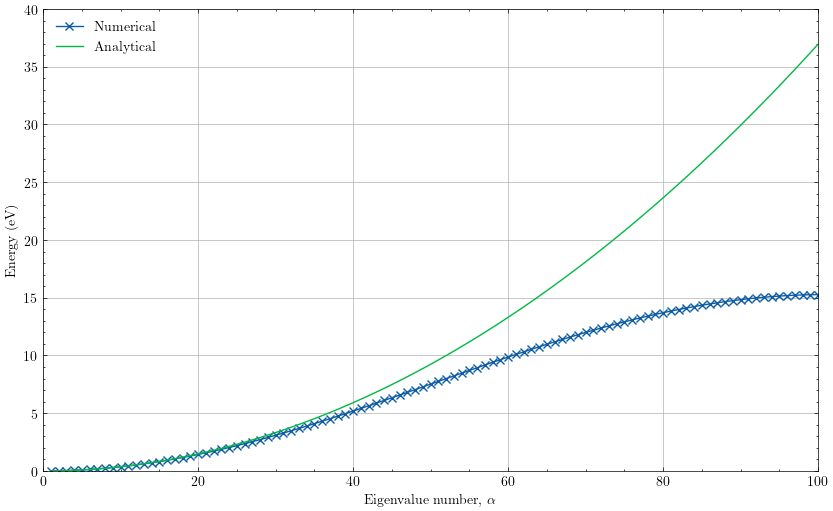
\includegraphics[scale=0.6]{discrete_PIB.png}
\caption{\textit{Numerical evaluation yields 100 eigenvalues that follow the analytical result well for low energies but deviate at higher energies because the wavefunctions oscillate too rapidly.}}\label{discrete_PIB}
\end{figure}

\vspace{1cm}

The process of discretization did not yield an accurate analytical answer in this case since the setup itself is intrinsically continuous. However, for the problems we are interested in, this process yields fairly accurate solutions since the periodic nature of the lattice then facilitates its description as a discretized system. 

\clearpage

\subsection{Toy Examples}

Consider a toy one-dimensional solid composed of $N$ atoms, separated by a distance $a$. Assuming one orbital per atom and periodic boundary condition, the $N\times N$ Hamiltonian matrix can be written as follows:

\begin{equation}
H =
\begin{matrix}
     & \ket{1} & \ket{2} & \ldots & \ket{N-1} & \ket{N} \\
    \ket{1} & E_0 & E_{ss} & \ldots & 0 & E_{ss} \\
    \ket{2} & E_{ss} & E_0 & \ldots & 0 & 0 \\
    \vdots  &  &  &  &  &  \\
    \ket{N-1} & 0 & 0 & \ldots & E_0 & E_{ss} \\
    \ket{N} & E_{ss} & 0 & \ldots & E_{ss} & E_0 \\
\end{matrix}   
\end{equation}

The off-diagonal elements at the top-right and the bottom-left are to account for the fact that we are applying the \textit{periodic boundary condition}. The set of equations (all identical in form) that we obtain by applying $[H]\psi = E\psi$ can be written as ($n = 1, 2,\ldots N$)
\begin{equation*} \label{toy_prob}
    E\psi_{n} = E_0\psi_{n} + E_{ss}\psi_{n-1} + E_{ss}\psi_{n+1}
\end{equation*}

This set of equations can be solved analytically by the ansatz (via Bloch's Theorem):
\begin{equation*} 
    \psi_{n} = \psi_0 e^{ikna} \quad \text{where} \quad ka = n2\pi/N
\end{equation*}

Substituting the ansatz into \ref{toy_prob}, we obtain
\begin{equation}
    E = E_0 + 2E_{ss}cos(ka)
\end{equation}

It would seem logically inconsistent that while we started out with a $N \times N$ Hamiltonian and were expected to find $N$ discrete eigenvalues, we have instead found a continuous, periodic function apparently implying that we have infinitely many possible eigenvalues. However, there is something more subtle at work here - due to the discrete nature of the lattice, values of $ka$ that differ by $2\pi$ represent identical states, which can be verified by considering the ansatz ($k^{'} = k + 2\pi/a$):

\begin{equation*}
\begin{aligned}
    \psi_{n}^{'} &= \psi_{0}e^{ik^{'}na} = \psi_{0}e^{ikna}e^{in2\pi} \\
    \psi_{n}^{'} &= \psi_{0}e^{ikna} = \psi_{n}
\end{aligned}
\end{equation*}

Since only the values of $ka$ within a range of $2\pi$ yield independent solutions, in principle, we could take any range of size $2\pi$, and it would be physically acceptable. It is common to restrict $ka$ to the range $-\pi < ka < \pi$, otherwise known as the first Brillouin zone. Note that while we have now limited the possible eigenvalues within the first BZ, the continuous function seemingly implies that there are still infinitely many eigenvalues within the zone itself. This issue can be resolved by taking into consideration the periodic boundary condition applied to the Hamiltonian initially: $\psi_{0} = \psi_{N}$. This implies

\begin{equation*}
\begin{aligned}
    \psi_{0} &= \psi_{N} = \psi_{0}e^{ikNa} \\
    ka &= \frac{2\pi}{N}\nu
\end{aligned}  
\end{equation*}

where $\nu \in Z$. Thus, we end up with $N$ discrete energy eigenvalues, all bound within the first Brillouin zone, as intended from physical intuition.

\vspace{1cm}

\begin{figure}[h]
\centering
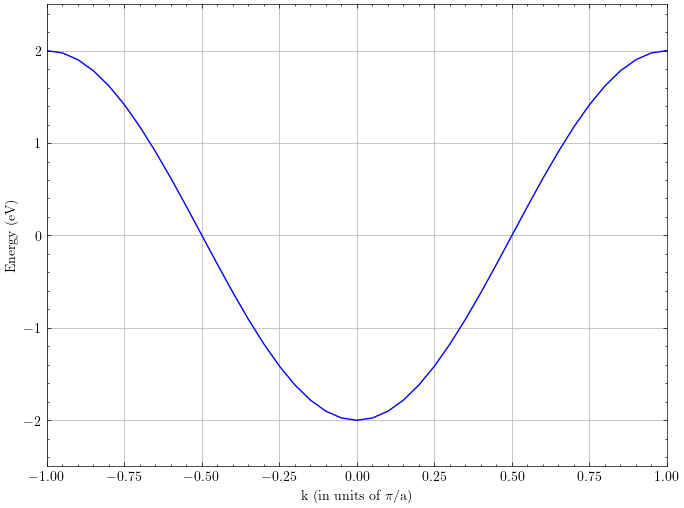
\includegraphics[scale=0.6]{1D_chain.png}
\caption{\textit{Bandstructure for a one-dimensional solid with $E_0 = 0$ and $E_{ss} = -1$.}}
\end{figure}

\vspace{1cm}

 % Bandstructure 

\chapter{Transport Phenomena in Semiconductor-Superconductor Hybrid Structures}

The non-equilibrium Green's function (NEGF) technique has emerged as a powerful tool for modelling nanoscale devices. Due to the versatility of the NEGF formalism, it can also be employed for devices that incorporate superconducting elements, which are of great academic interest, especially ones involving topological superconductivity and Majorana bound states. Refer to Appendix~\ref{appendix:NEGF} for a brief discussion of the NEGF formalism used throughout the text. \par 

\section{The Bogoliubov deGennes Hamiltonian}

The {\bf B}ardeen-{\bf C}ooper-{\bf S}chreiffer theory was presented in 1956 as a variational mean-field approach to phonon-mediated inter-electron attractive interactions, leading to the formation of Cooper pairs below a critical temperature. As a superconductor is cooled below its critical temperature, the attractive interactions between electrons dominate over the repulsive Coulombic forces. In the presence of a net-attractive interaction, no matter how weak, the normal metal state becomes unstable. An attractive matrix element can arise by the coupling of electrons to another system of particles or excitations in the solid. The BCS theory was the first microscopic description of the ground state of the superconductor, following which Bogoliubov formulated a concise framework in terms of quasiparticles to describe setups which feature superconductors coupled with normal systems. \par 

A system of interacting electrons is described by the second quantization Hamiltonian, in terms of electron creation (annihilation) field operators $\Psi^{\dagger}(\textbf{r}\sigma)$ ($\Psi(\textbf{r}\sigma)$), at position $\textbf{r}$, with spin $\sigma$

\begin{equation}
        \begin{aligned}
        H &= \underbrace{H_{0}}_{\text{single-particle Hamiltonian}} +\underbrace{H_{int}}_{\text{four-fermion interaction Hamiltonian}} \\
        H_{0} &= \int d\textbf{r} \sum_{\sigma} \Psi^{\dagger}(\textbf{r}\sigma) \left[ \frac{(-i\hbar \nabla - e \textbf{A})^{2}}{2m^{*}} + U_{0}(\textbf{r}\sigma) - \mu \right] \Psi(\textbf{r}\sigma) \\
        H_{int} &= -\frac{1}{2}V \int d\textbf{r} \sum_{\sigma, \sigma'} \Psi^{\dagger}(\textbf{r}\sigma) \Psi^{\dagger}(\textbf{r}\sigma') \Psi(\textbf{r}\sigma') \Psi(\textbf{r}\sigma)
        \end{aligned}
\end{equation}
 
where $\textbf{A}$ is the magnetic vector potential, $m^{*}$ is the electron effective mass, $U_{0}$ is the single-particle potential energy and $V$ scales the interaction energy. Using the mean-field approximation, the four-fermion interaction potential can be expressed as an average potential acting on one particle at a time, which restricts the Hamiltonian to terms quadratic in field operators.

\begin{equation*}
        H_{mf} = \int d\textbf{r} \sum_{\sigma}\Psi^{\dagger}(\textbf{r}\sigma)[H_{0}+U_{\sigma}]\Psi(\textbf{r}\sigma) + \int d\textbf{r} \: [\Delta \: \Psi^{\dagger}_{\uparrow} \Psi^{\dagger}_{\downarrow} + \Delta^{*} \: \Psi_{\downarrow} \Psi_{\uparrow}]
\end{equation*}

The superconducting order parameter ($\Delta$), which couples electrons and holes of opposite spin and momentum, is the physical quantity that sets apart superconductors from a normal insulator. Apart from the conventional terms involving Coulomb interaction, which are of the form $\langle \psi_{i}^{\dagger}\psi_{j} \rangle$ (where $i$, $j$ are labelling indices for a combination of quantum-state and spin), there are anomalous terms of the form $\langle \psi_{i}^{\dagger}\psi_{j}^{\dagger} \rangle$ arising from the Cooper pairing process below the critical temperature. \par 

As per the BCS theory, the indices can be transformed as $i \rightarrow k \uparrow$, and $j \rightarrow -k \downarrow$ for a continuum model. Assuming a metallic system, we end up with up-spin and down-spin bands filled up to the Fermi level designated by the electrochemical potential $\mu$. A ``hole'' transformation can be performed on the down-spin band, which flips the band, and the down-spins are now represented by unfilled particles or holes, similar to semiconductor physics. This is equivalent to a 2-component spinor transformation:

\begin{equation}
    \begin{bmatrix}
        \Psi^{\dagger}_{\uparrow}(\textbf{r}) \\
        \Psi^{\dagger}_{\downarrow}(\textbf{r})
     \end{bmatrix} \rightarrow
     \begin{bmatrix}
        \Psi^{\dagger}_{\uparrow}(\textbf{r})\\
        \Psi_{\downarrow}(\textbf{r})
     \end{bmatrix} (\text{in real space}), \: 
     \begin{bmatrix}
        c^{\dagger}_{k \uparrow} \\
        c^{\dagger}_{-k \downarrow}    
     \end{bmatrix} \rightarrow
     \begin{bmatrix}
        c^{\dagger}_{k\uparrow} \\
        c_{-k\downarrow}   
     \end{bmatrix} (\text{in \textit{k}-space})
\end{equation}

The Hamiltonian of the continuum model is a $2 \times 2$ matrix in $k$-space, with two dispersion relations that get coupled due to the pairing term $\Delta_{k}$.

\begin{equation*}
    H_{k} = \begin{bmatrix}
            (\epsilon_{k}-\mu) & \Delta_{k} \\
            \Delta^{*}_{k} & -(\epsilon_{k}-\mu)
    \end{bmatrix}
\end{equation*}

where, $\epsilon_{k} = \frac{\hbar^{2}k^{2}}{2m^{*}}$. \par 

We can discretise the continuum model described above into a lattice model with a spacing of $a$. The on-site component of the Hamiltonian is given as 

\begin{equation}
    \alpha_{S} = \begin{bmatrix}
          2t-\mu & \Delta_{0} \\
          \Delta_{0}^{*} & -(2t-\mu)  
    \end{bmatrix}
\end{equation}

where, $t = \frac{\hbar^{2}}{2m^{*}a^{2}}$ is the nearest-neighbour hopping parameter. The nearest-neighbour hopping matrix is given by 

\begin{equation}
    \beta = \begin{bmatrix}
          -t & 0\\
          0 & t  
    \end{bmatrix}    
\end{equation}

The tight-binding Hamiltonian is subsequently written as

\begin{equation}
    H = \sum_{i}^{N}c^{\dagger}_{i}\alpha_{S}c^{i} + \sum_{i\neq j}^{N}c^{\dagger}_{i}\beta c_{j}    
\end{equation}

where $c^{\dagger}_{i}$ is the creation operator of the Nambu 2-component spinor ar site $i$, and $N$ is the number of sites in the device. The Hamiltonian of the superconducting sample can be written in the general form 

\begin{equation}
H = \begin{pmatrix}
\alpha_S & \beta & 0 & \dots & 0 \\
\beta^{\dagger} & \alpha_S & \beta & 0 & 0 \\
0 & \beta^{\dagger} & \alpha_S & \beta & \vdots \\
\vdots & 0 & \ddots & \ddots & \beta \\
0 & \dots & \dots & \beta^{\dagger} & \alpha_S \\
\end{pmatrix}   
\end{equation}


\section{The Isolated Kitaev Chain}

The field of topological superconductivity began with a lattice model proposed by Kitaev in 2001. The Kitaev chain is a tight-binding chain of $N$ lattice sites, with one spinless fermionic orbital at each site and nearest-neighbour $p$-wave superconducting pairing. The $p$-wave nature of the superconductivity couples particles of equal spin, allowing a spinless treatment. The pairing is treated in the usual mean-field approach, yielding the Kitaev grandcanonical Hamiltonian

\begin{equation}
    \hat{H}_{\text{KC}} = -\mu \sum_{j=1}^{N}c^{\dagger}_{j}c_{j} - t\sum_{j=1}^{N-1}(c^{\dagger}_{j+1}c_{j}+c^{\dagger}_{j}c_{j+1})-\Delta \sum_{j=1}^{N-1}(c^{\dagger}_{j}c^{\dagger}_{j+1}+c_{j+1}c_{j})    
\end{equation}

in terms of the fermionic creation (annihilation) field operators $c^{\dagger}_{j}$ ($c_{j}$). The hopping amplitude $t$ and the superconducting pairing constant $\Delta$ are assumed to be real quantities in this case. The chemical potential $\mu$ represents the on-site energy and can be modulated by applying a gate voltage. \par 

The Kiteav Hamiltonian has been of particular interest in the context of topological superconductivity due to the possibility of hosting Majorana zero modes (MZMs) at its end in a particular parameter range. This can be seen by expressing the Hamiltonian in terms of so-called Majorana operators $\gamma^{A,B}$,

\begin{equation}
    \begin{pmatrix}
        c_{j} \\
        c^{\dagger}_{j}    
    \end{pmatrix} = \frac{1}{\sqrt{2}}
    \begin{pmatrix}
        \gamma^{A}_{j} \\
        \gamma^{B}_{j}    
    \end{pmatrix}, \: (\gamma^{A,B})^{\dagger} = \gamma^{A,B},
\end{equation}

yielding the form

\begin{equation} \label{eq:majorana}
    \hat{H}_{\text{KC}} = -i\mu \sum_{j=1}^{N}\gamma^{A}_{j}\gamma^{B}_{j} + i(\Delta+t)\sum_{j=1}^{N-1}\gamma^{B}_{j}\gamma^{A}_{j+1}+i(\Delta-t)\sum_{j=1}^{N-1}\gamma^{A}_{j}\gamma^{B}_{j+1}  
\end{equation}

For the particular parameter settings $\Delta = \pm t$ and $\mu = 0$, which we call the Kitaev points, equation (\ref{eq:majorana}) leads to a `missing' fermionic quasiparticle $q_{\pm}$ at the extrema of the Kitaev chain:

\begin{equation}
    \begin{aligned}
       q_{+} &= \frac{1}{\sqrt{2}}(\gamma^{A}_{1}+i\gamma^{B}_{N}) \quad [\Delta = t] \\
       q_{-} &= \frac{1}{\sqrt{2}}(\gamma^{B}_{1}+i\gamma^{A}_{N}) \quad [\Delta = -t]          
    \end{aligned}    
\end{equation}

This quasiparticle has zero energy and is composed of two isolated Majorana states localised at the ends of the chain. In general, the condition of hosting MZM is not restricted to the Kitaev points. \par

\subsection{Bulk spectrum}

The Kitaev Hamiltonian in the limit of $N \rightarrow \infty$ reads in $k$-space 

\begin{equation*}
    \hat{H}_{\text{KC}} = \frac{1}{2}\sum_{k}\hat{\psi}^{\dagger}_{k}H(k)\hat{\psi}_{k}, \quad \hat{\psi}^{\dagger}_{k} = \begin{pmatrix}
       c_{k} & c_{-k}^{\dagger}     
    \end{pmatrix}^{\text{T}}     
\end{equation*}

The $2 \times 2$ BdG matrix

\begin{equation}
    H(k) = 
    \begin{bmatrix}
       -\mu-2t\:\text{cos}(ka) & -2i\Delta \: \text{sin}(ka) \\
       2i\Delta \: \text{sin}(ka) & \mu+2t\: \text{cos}(ka)         
    \end{bmatrix}    
\end{equation}

can be diagonalized to yield the excitation spectrum

\begin{equation}
    E_{\pm}(k) = \pm \sqrt{4\Delta^{2}\:\text{sin}^{2}(ka)+[\mu+2t\: \text{cos}(ka)]^{2}}    
\end{equation}

\subsection{Energy spectrum of the finite Kitaev chain}

Next, consider a finite Kitaev chain with $N$ sites and open boundary conditions, yielding $N$ allowed $k$ values. The BdG Hamiltonian of the open Kitaev chain can be expressed in the basis of standard fermionic operators $\hat{\psi} = (c_{1},\dots,c_{N},c_{1}^{\dagger},\dots,c_{N}^{\dagger})$,

\begin{equation*}
    \hat{H}_{\text{KC}} = \frac{1}{2}\hat{\psi}^{\dagger}H_{\text{KC}}\hat{\psi}     
 \end{equation*}

 where the BdG Hamiltonian $H_{\text{KC}}$ is

 \begin{equation}
     H_{\text{KC}} = \begin{bmatrix}
          C & S \\
          S^{\dagger} & -C   
     \end{bmatrix}     
 \end{equation} 

 These matrices have the tridiagonal structure

\begin{equation}
    \begin{aligned}
        C &= 
        \begin{bmatrix}
        -\mu & -t &  &  &  &  &  \\
        -t & -\mu & -t &  &  &  &  \\
         & -t & -\mu & -t &  &  &  \\
         &  & \ddots & \ddots & \ddots &  &  \\
         &  &  & -t & -\mu & -t &  \\
         &  &  &  & -t & -\mu & -t \\
         &  &  &  &  & -t & -\mu \\
        \end{bmatrix}_{N \times N} \\
        S &= 
        \begin{bmatrix}
        0 & \Delta &  &  &  &  &  \\
        -\Delta & 0 & \Delta &  &  &  &  \\
         & -\Delta & 0 & \Delta &  &  &  \\
         &  & \ddots & \ddots & \ddots &  &  \\
         &  &  & -\Delta & 0 & \Delta &  \\
         &  &  &  & -\Delta & 0 & \Delta \\
         &  &  &  &  & -\Delta & 0 \\              
        \end{bmatrix}_{N \times N}      
    \end{aligned} 
\end{equation}

the spectrum can be obtained by diagonalising $H_{\text{KC}}$ in real space. The fermionic operators associated with the Kitaev chain can be represented in several bases, each suited to facilitate some specific calculation. The default basis can be rearranged to a site-ordered particle-hole basis where $\hat{\psi} = (c_{1}^{\dagger},c_{1},\dots,c_{N}^{\dagger})$ with the BdG Hamiltonian matrix given by 

\begin{equation}
    H_{\text{KC}} = 
    \begin{bmatrix}
        \alpha & \beta &  &  &  &  &  \\
        \beta^{\dagger} & \alpha & \beta &  &  &  &  \\
        & \beta^{\dagger} & \alpha & \beta &  &  &  \\
        &  & \ddots & \ddots & \ddots &  &  \\
        &  &  & \beta^{\dagger} & \alpha & \beta &  \\
        &  &  &  & \beta^{\dagger} & \alpha & \beta \\
        &  &  &  &  & \beta^{\dagger} & \alpha \\        
    \end{bmatrix}_{N \times N}   
\end{equation}

where 

\begin{equation}
    \begin{aligned}
        \alpha &= 
        \begin{bmatrix}
            -\mu & 0 \\
            0 & \mu            
        \end{bmatrix}, \\
        \beta &= 
        \begin{bmatrix}
            -t & \Delta \\
            -\Delta & t             
        \end{bmatrix}        
    \end{aligned}    
\end{equation}

\clearpage

\vspace*{1cm}

\begin{figure}[h]
\centering
\includegraphics[scale=0.55]{KC.png}
\caption{\textit{Eigenspectrum of the finite Kitaev chain as a function of $\mu/\Delta$ for N = 25, $\Delta/t = 1.0$. Note the zero energy modes observed within the topological regime, i.e., $|\mu| < 2|t|$.}}
\end{figure}

\vspace{1cm}

We can also construct a ``disordered'' system with local inhomogeneity in the on-site potential. Such an inhomogeneity might occur due to Fermi energy mismatch as well as charge inhomogeneities in the system. For the disordered chain, the zero energy modes are observed both in the topological regime and in the trivial regime, which can make it difficult to identify genuine topological transitions in an experimental scenario.

\clearpage

\vspace*{2cm}

\begin{figure}[!htbp]
\centering
\includegraphics[scale=0.4]{KC_pristine_spectrum_21.png}
\caption{\textit{Eigenspectrum for a pristine setup with $N = 21$ and $t/\Delta = 4.1$}}
\vspace{1cm}
\includegraphics[scale=0.4]{KC_disorder_spectrum_21.png}
\caption{\textit{Eigenspectrum for a disordered setup with $N = 21$ and $t/\Delta = 4.1$}}
\end{figure}    

\clearpage

\vspace*{2cm}

\begin{figure}[!htbp]
\centering
\includegraphics[scale=0.4]{KC_pristine_spectrum_100.png}
\caption{\textit{Eigenspectrum for a pristine setup with $N = 100$ and $t/\Delta = 4.1$}}
\vspace{1cm}
\includegraphics[scale=0.4]{KC_disorder_spectrum_100.png}
\caption{\textit{Eigenspectrum for a disordered setup with $N = 100$ and $t/\Delta = 4.1$}}
\end{figure} 

\clearpage


\section{Voltage Driven Transport}

Andreev processes are fundamental to our understanding of transport phenomena across superconducting hybrid devices. They involve the reflection of an electron (hole) as a spin-reversed hole (electron), resulting in the transfer of a Cooper pair in the superconductor. Andreev reflections arise naturally from the BdG Hamiltonian, which has the form as shown in equation (\ref{eq:BdG}), and are thus characteristic processes of an N/S interface and are absent in normal junctions.

\begin{equation} \label{eq:BdG}
    H_{\text{BdG}} = \begin{bmatrix}
            H_{\uparrow}+U-\mu & \Delta \\
            \Delta^{*} & -(H_{\downarrow}+U-\mu)
    \end{bmatrix}    
\end{equation}

where $H_{\uparrow(\downarrow)}$ refers to the Hamiltonian of the up- (down)-spin sector, and $U$ refers to the local potentials that give rise to various reflection and transmission processes. The order parameter $\Delta$ can be viewed as a potential which couples the up-spin (upper) block with the down-spin (lower) block and is responsible for Andreev processes. 

\vspace{1cm}

\begin{figure}[h]
\centering
\includegraphics[scale=0.85]{andreev_reflection.png}
\caption{\textit{Andreev Reflection -- An incoming electron from the normal region is reflected as a spin-reversed hole, resulting in the transfer of a Cooper pair into the superconductor.}}
\end{figure}

\vspace{1cm}

Therefore, in superconducting systems, we end up with two distinct processes -- normal reflections, wherein electrons and holes reflect independently, and Andreev reflections, where electrons (holes) can reflect off as spin-reversed holes (electrons). 

\clearpage 

\subsection{N/S Junctions} \label{subsec:NS}

In the ballistic regime, we are familiar with the conductance quantisation in normal insulators, where each mode conducts with a conductance $G = \frac{2e^{2}}{h}$. However, as a consequence of Andreev processes, the conductance quantum is doubled in an N/S interface in the so-called ``sub-gap'' regime. Similar to the regular barrier potential in normal devices, which serve as a gap for the transmission of electrons/holes, the order parameter $\Delta$ can be thought of as a barrier in the superconducting region, which implies that the energy range $-\Delta < E < \Delta$ is unique to Andreev processes. \par 

In the electron-hole Nambu space, each contact has two components: the electron and the hole blocks. Assuming that a bias voltage $V$ is impressed on the N-side while the S-side is kept grounded, the electronic electrochemical potential translates to $\mu_{\text{N}e} = +eV$, and the hole electrochemical potential translates to $\mu_{\text{N}h} = -eV$. In layman's terms, it is as if the contact splits into two viable contacts simply as a result of the BdG framework being used to describe the junction. \par 

This can also be explained in more mathematical detail via the NEGF framework. The contact broadening matrices can be written with a general diagonal structure (due to diagonal structure of normal contacts in the Nambu space) as $\Gamma_{\alpha} = \Gamma_{\alpha}^{ee} + \Gamma_{\alpha}^{hh}$, where the superscripts $ee \: (hh)$denote the electron (hole) diagonal component of the broadening matrix, and $\alpha = \text{L/R}\/\text{N/S}$. The current across the N/S junction can be derived from the electron or hole current at the N-contact as,

\begin{equation} \label{eq:NS}
   \begin{aligned}
       I^{e(h)}_{N}(E) &= \frac{e}{h}\left(\underbrace{\textbf{Tr}(\Gamma_{L}^{ee(hh)}G^{r}\Gamma_{R}^{ee(hh)}G^{a})}_{T_{D}}\:[f_{N}^{ee(hh)}(E)-f_{S}^{ee(hh)}(E)]\right)  \\
       &+ \frac{e}{h}\left(\underbrace{\textbf{Tr}(\Gamma_{L}^{ee(hh)}G^{r}\Gamma_{L}^{hh(ee)}G^{a})}_{T_{A}}\:[f_{N}^{ee(hh)}(E)-f_{N}^{hh(ee)}(E)]\right)         
   \end{aligned}       
\end{equation}  

where the first term represents the direct transmission process of electron (hole), the second term represents the direct Andreev transmission, and the Fermi distributions are denoted by $f^{ee}_{\alpha}=f(E-\mu_{\alpha})$, $f^{hh}_{\alpha}=f(E+\mu_{\alpha})$. \par 

Given the fact that the total current (electron + hole) is double that of each sector as defined in equation (\ref{eq:NS}), the current at the N-side can be expressed in a more concise form as,

\begin{equation}
    I_{N} = \frac{2e}{h}\int dE\:(T_{D}(E)\:[f(E-eV)-f(E)]+T_{A}(E)\:[f(E-eV)-f(E+eV)])    
\end{equation}

From the above equation, one can analytically evaluate the current by setting the temperature $T \rightarrow 0$, and taking derivatives w.r.t. the applied bias at the N-side. In the sub-gap regime, Andreev transmission dominates with a probability of unity since the superconducting segment is infinitely long. From this, we get $G(V) = \frac{\partial I_{N}}{\partial V} = \frac{4e^{2}}{h}$, elucidating the conductance doubling in the sub-gap regime. In the supra-gap regime, Andreev transmission occurs alongside direct transmission, which gives a conductance $G(V) = \frac{4e^{2}}{h}T_{A} + \frac{2e^{2}}{h}T_{D}$, with a suppression of $T_{A}$ with increasing bias voltage. In the asymptotic range of large energies, only the direct transmission dominates due to the quasiparticle transmission and this leads to a conductance of $\frac{2e^{2}}{h}$ at large bias. \par 

\vspace{3cm}

\begin{figure}[h]
\centering
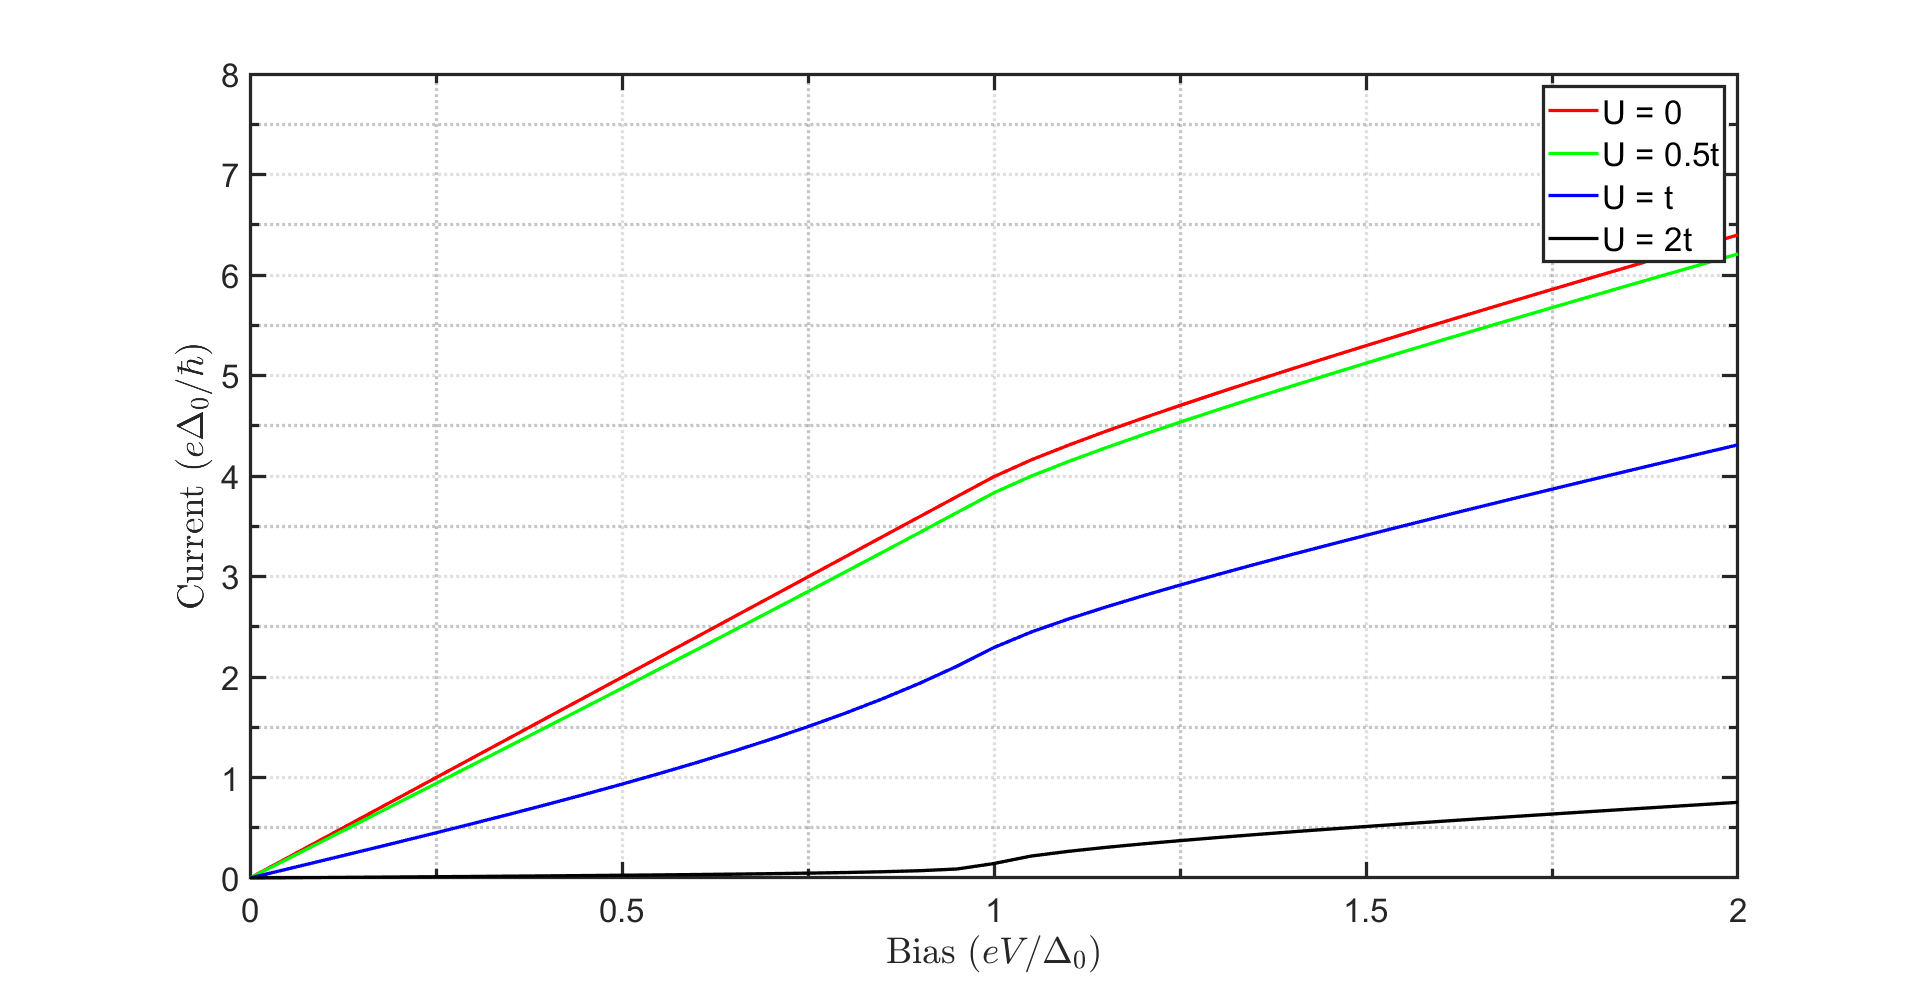
\includegraphics[scale=0.3]{I-V.png}
\caption{\textit{Current as a function of the applied bias across an N/S junction.}}
\end{figure}

\clearpage

\begin{figure}[h]
\centering
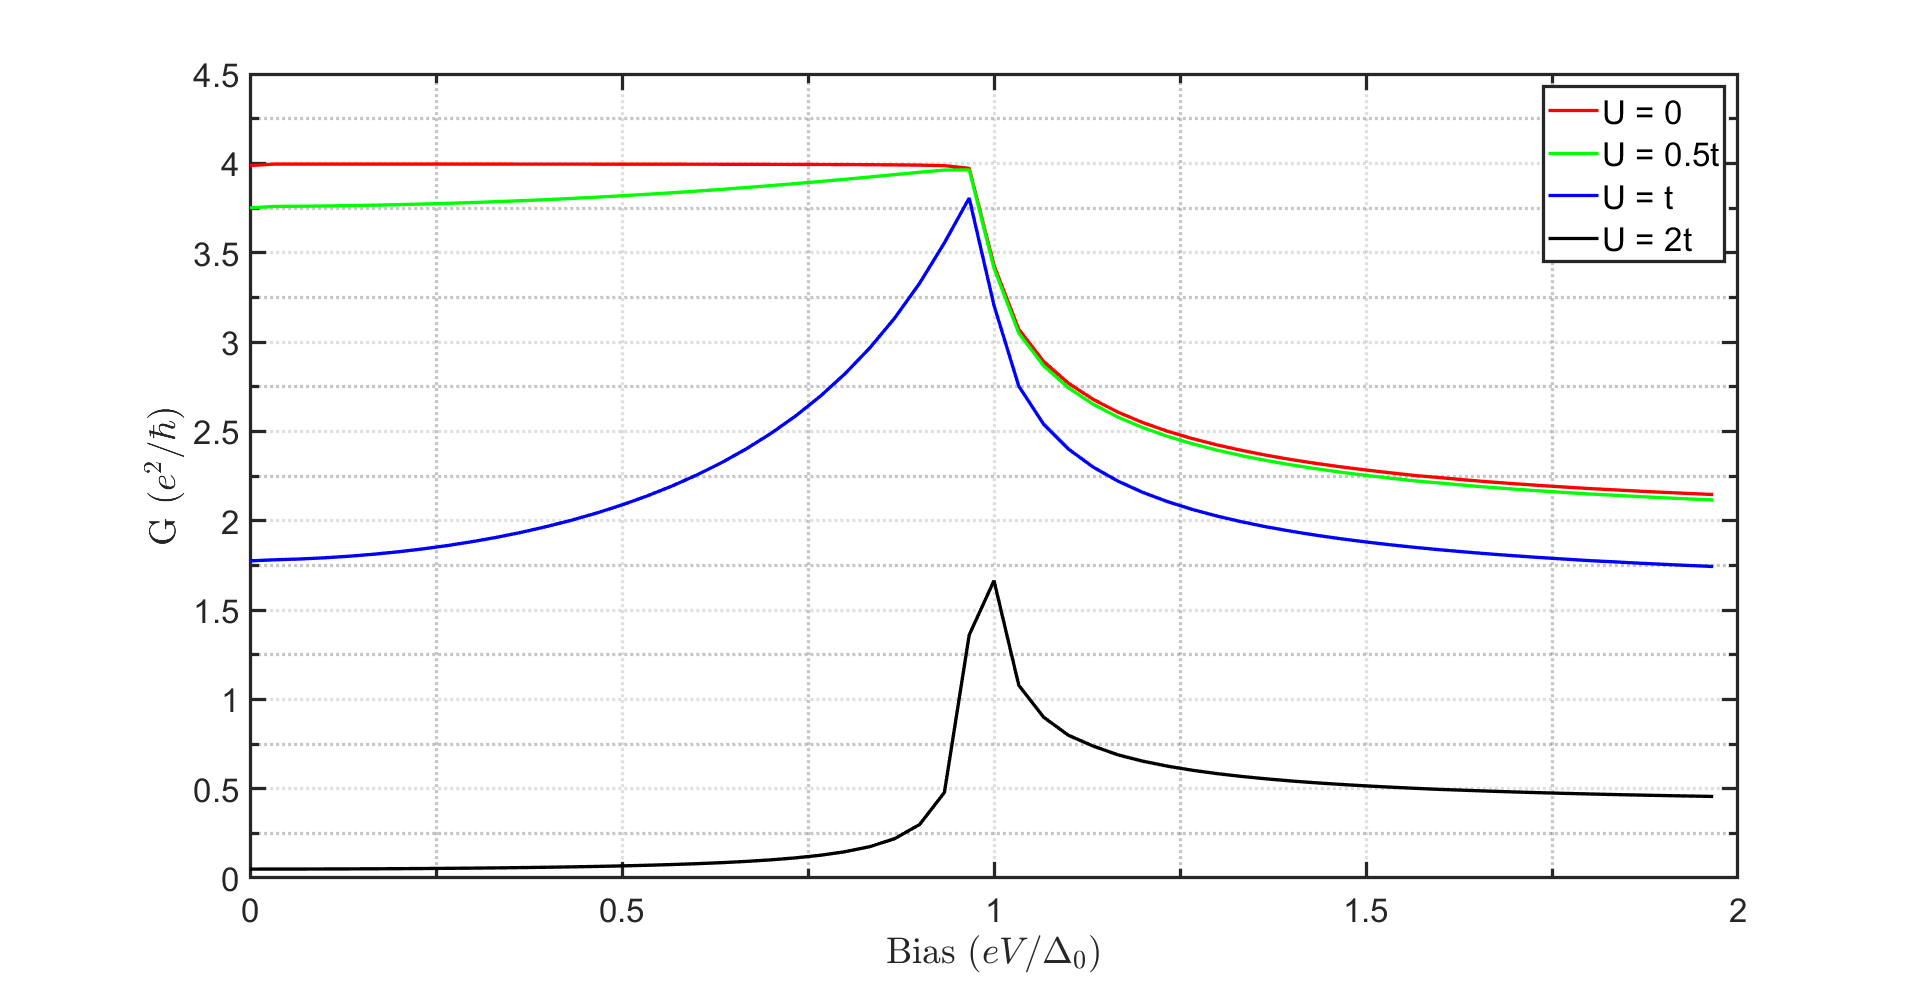
\includegraphics[scale=0.3]{G-V.png}
\caption{\textit{Conductance as a function of the applied bias across an N/S junction.}}
\end{figure}

\vspace{1cm}

A potential $U$ of varying magnitude has been introduced in the numerical simulations to simulate imperfect interfaces, which relates to the ``transparency'' of the interface. As $U$ increases, the sub-gap Andreev processes are suppressed, with increasing dominance of the direct reflection processes.


\subsection{N-S-N Structure}

In an N-S-N setup, we have two N-S interfaces, with the superconducting region acting as the device region and the two N-regions as contacts. Similar to the Fabry-Perot resonance in double barrier devices, multiple Andreev reflections give rise to resonant states termed as \textit{Andreev bound states} (ABS). The superconducting region, in particular, would be a finite Kitaev chain, which is contacted on both sides with normal leads for the remainder of this text. \par 

As discussed in \ref{subsec:NS}, the N/S junction can be visualised as two independent terminals operating at the same contact. Following from this argument, the analysis of the N-S-N setup will be based on an elaborate four-terminal device based on the Landauer-Büttiker setup. Apart from the generic direct and Andreev transmission processes, we now have an additional Andreev process termed as the crossed Andreev reflection (CAR), which corresponds to the transmission of an electrons (holes) from the left (right) contact as a hole (electron) from the right (left) contact. We can express the current across the system as a sum of three components,

\begin{equation}
    \begin{aligned}
        I^{e(h)}_{L}(E) &= \frac{e}{h}\left(\underbrace{\textbf{Tr}(\Gamma_{L}^{ee(hh)}G^{r}\Gamma_{R}^{ee(hh)}G^{a})}_{T_{D}}\:[f_{L}^{ee(hh)}(E)-f_{R}^{ee(hh)}(E)]\right)  \\
       &+ \frac{e}{h}\left(\underbrace{\textbf{Tr}(\Gamma_{L}^{ee(hh)}G^{r}\Gamma_{L}^{hh(ee)}G^{a})}_{T_{A}}\:[f_{L}^{ee(hh)}(E)-f_{L}^{hh(ee)}(E)]\right) \\
       &+ \frac{e}{h}\left(\underbrace{\textbf{Tr}(\Gamma_{L}^{ee(hh)}G^{r}\Gamma_{R}^{hh(ee)}G^{a})}_{T_{CAR}}\:[f_{L}^{ee(hh)}(E)-f_{R}^{hh(ee)}(E)]\right)
    \end{aligned}    
\end{equation}

where the third term represents the CAR process. \par 

In order to setup the transport simulations, we can potentially by-pass the tedious surface Green's function calculations by making the wide-band approximation, such that a constant density of states is assumed in the energy range of interest. This results in a constant $\gamma$ value for each relevant element of the broadening matrix $\Gamma$. \par 

Since we have two N-S interfaces, one can apply a bias across the device with a generic condition on $\mu_{L}$ and $\mu_{R}$. This can prove useful during numerical simulations, since applying a symmetric bias of $V_{L} = -V_{R} = V/2$ will nullify the crossed Andreev reflection term, $T_{CAR}$. \par 

\vspace{1cm}

\begin{figure}[h]
\centering
\includegraphics[scale=0.7]{KC_conductance.png}
\caption{\textit{Total linear conductance ($G_{A}+G_{D}$) in units of $e^{2}/h$ for $N = 20, \gamma_{L/R}/\Delta = 0.001$ as a function of $\mu/\Delta$.}}
\end{figure}

\clearpage 

\vspace*{1.5cm}

\begin{figure}[h]
\centering
\includegraphics[scale=0.65]{KC_Nsites_var.png}
\caption{\textit{Total linear conductance ($G_{A}+G_{D}$) in units of $e^{2}/h$ for $\mu = 0.0, \gamma_{L/R}/\Delta = 0.001$ as a function of $N$.}}
\end{figure}

\vspace{0.6cm}

\begin{figure}[h]
\centering
\includegraphics[scale=0.65]{KC_resonant_modes.png}
\caption{\textit{Resonant modes in the linear conductance after $t/\Delta$ exceeds a threshold value.}}
\end{figure}

\clearpage

\subsubsection{Linear Transport}

In the linear transport regime ($V \rightarrow 0, T \rightarrow 0$), the closed form expressions for the conductance of the Kitaev chain have been simulated with reference to \cite{transport_paper}. 

\vspace{0.6cm}

\begin{figure}[h]
\centering
\includegraphics[scale=0.7]{KC_GD_cmap.png}
\caption{\textit{Direct conductance term ($G_{D}$) in units of $e^{2}/h$ for $\gamma_{L/R}/\Delta = 0.001$ as a function of $\mu/\Delta$ and $t/\Delta$.}}
\end{figure}

\vspace{0.5cm}

\begin{figure}[h]
\centering
\includegraphics[scale=0.7]{KC_GA_cmap.png}
\caption{\textit{Andreev conductance term ($G_{A}$) in units of $e^{2}/h$ for $\gamma_{L/R}/\Delta = 0.001$ as a function of $\mu/\Delta$ and $t/\Delta$.}}
\end{figure}

\clearpage

\vspace*{3cm}

\begin{figure}[h]
\centering
\includegraphics[scale=1.0]{KC_Gtot_cmap.png}
\caption{\textit{Total conductance ($G_{A}+G_{D}$) in units of $e^{2}/h$ for $\gamma_{L/R}/\Delta = 0.001$ as a function of $\mu/\Delta$ and $t/\Delta$.}}
\end{figure}

\clearpage 

\subsubsection{Non-linear Transport} 

\vspace*{3cm}

\begin{figure}[h]
\centering
\includegraphics[scale=0.5]{pristine_transport_0.png}
\caption{\textit{Differential conductance of a pristine setup in units of $e^{2}/h$ as a function of $eV/2\Delta$ and $\mu/\Delta$ for $N = 21, \gamma_{L/R}/\Delta = 0.02$, and $|t/
\Delta| = 4.1$.}}
\end{figure}

\clearpage 

\vspace*{3cm}

\begin{figure}[h]
\centering
\includegraphics[scale=0.5]{disorder_transport_0.png}
\caption{\textit{Differential conductance of a disordered setup in units of $e^{2}/h$ as a function of $eV/2\Delta$ and $\mu/\Delta$ for $N = 21, \gamma_{L/R}/\Delta = 0.02$, and $|t/
\Delta| = 4.1$.}}
\end{figure}

\clearpage 

\vspace*{3cm}

\begin{figure}[h]
\centering
\includegraphics[scale=0.5]{pristine_transport_1.png}
\caption{\textit{Differential conductance of a pristine setup in units of $e^{2}/h$ as a function of $eV/2\Delta$ and $\mu/\Delta$ for $N = 21, \gamma_{L/R}/\Delta = 0.02$, and $|t/
\Delta| = 1.0$.}}
\end{figure}

\clearpage 

\vspace*{3cm}

\begin{figure}[h]
\centering
\includegraphics[scale=0.5]{disorder_transport_1.png}
\caption{\textit{Differential conductance of a disordered setup in units of $e^{2}/h$ as a function of $eV/2\Delta$ and $\mu/\Delta$ for $N = 21, \gamma_{L/R}/\Delta = 0.02$, and $|t/
\Delta| = 1.0$.}}
\end{figure} % Transport phenomena in SC hybrid structures

%% ----------------------------------------------------------------
% Now begin the Appendices, including them as separate files

\addtocontents{toc}{\vspace{2em}} % Add a gap in the Contents, for aesthetics

\appendix % Cue to tell LaTeX that the following 'chapters' are Appendices

\chapter{Bloch's Theorem}

Periodic potentials are important in condensed matter physics, and we will be using the Bloch wavefunctions generously during the analysis of toy models. Secondly, periodic potentials will give us our first examples of Hamiltonian systems with symmetry, and they will serve to illustrate certain general principles of such systems. \par

We wish to solve the one-dimensional Schrödinger equation,

\begin{equation*}
    -\frac{\hbar^{2}}{2m}\psi^{\prime \prime} + V(x) \psi = E \psi
\end{equation*}

where the potential is assumed to be spatially periodic,

\begin{equation}
    V(x+a) = V(x)
\end{equation}

Here $a$ is the lattice spacing or spatial period of the 1-D lattice. No further assumptions need be made about the behaviour of $V(x)$ within any period apart from its periodicity. \par
Next, we shall make a strong assumption that there is a super-symmetry that rides over the good ole periodicity of the lattice points such that the lattice repeats itself after $N$ lattice spacings. This is equivalent to imposing a periodic/circular boundary condition on the solutions to the Hamiltonian. \par

We introduce the translation operator, $T(a)$, which has the effect of displacing the wave function by the lattice spacing $a$ along the x-axis. 

\begin{equation}
    T(a) \psi(x) = \psi (x-a)
\end{equation}

Functionally, the translation operator is given by,

\begin{equation}
    T(a) = e^{-\frac{iap}{\hbar}}
\end{equation}

An easy check will ascertain that this operator commutes with both kinetic energy, as well as potential energy operators. This means that \textit{T(a)} commutes with the entire Hamiltonian, 

\begin{equation}
    [T(a), H] = 0
\end{equation}

Put more generally, $H$ commutes with any power of $T(a)$, $T^{n}(a) = T(na)$, which is to say that it commutes with the entire group of symmetry operations generated by $T(a)$. \par

The fact that $H$ and $T(a)$ commute provides us a powerful tool to determine the eigenfunctions of $H$. More often than not, it is hard to find the eigenfunctions of $H$, but much easier to find those for the translation operator. Since we now know the eigenfunctions of the translation operator, it makes the search for the eigenfunctions of $H$ easier since they are a subset of the eigenspace of $T(a)$. \par

Since $T(a)$ is unitary, its eigenvalue $\tau$ must be a phase factor, $\tau = e^{-i\theta}$. The angle $\theta$ characterizes the eigenvalues of $T(a)$ and may be restricted to the range $-\pi < \theta \leq \pi$. It is conventional to write this angle in the form $\theta = ka$, where $k$ is a quantity with dimensions of wave number,
which characterizes the eigenvalue. We now have,

\begin{equation}
    T(a) \psi_{k}(x) = \psi_{k}(x-a) = e^{-ika}\psi_{k}(x)
\end{equation}

Equivalently, we can write this as,

\begin{equation}
\label{eq:bloch wavefunction}
    \psi_{k}(x+a) = e^{ika}\psi_{k}(x)
\end{equation}

Now we are faced with a dilemma - for any given value of $k$, there are functions $\psi_{k}$ which satisfy \ref{eq:bloch wavefunction}, so the spectrum of $T(a)$ is the entire unit circle in the complex plane. Furthermore, the number of such functions for any value of $e^{-ika}$ is infinite, so the eigenvalues are infinite-fold degenerate and the eigenspaces of $T(a)$ are infinite-dimensional. This would render the entire analysis using translation operators inconsequential since it was asserted that this approach would help limit the space in which we have to search for the eigenfunctions of $H$. This is exactly where the initial boundary condition assuming a super-symmetry comes into play. In case the lattice repeats itself after $N$ lattice spacings, the single-valuedness of the wavefunction requires

\begin{equation*}
    \psi(x+Na) = \psi(x)
\end{equation*}

so the eigenvalues of $T(a)$ are phase factors of the form $e^{-\frac{2n\pi i}{N}}$, for $n = 0,..., N-1$. In this case, the spectrum of $T(a)$ is discrete, although each eigenvalue is still infinite-fold degenerate. Rather than $\psi_{k}(x)$, it is often easier to work with a function $u_{k}(x)$, defined by

\begin{equation}
    \psi_{k}(x) = e^{ikx} u_{k}(x)
\end{equation}

where $u_{k}$ is periodic, $u_{k}(x+a) = u_{k}(x)$. \textit{Bloch's theorem} states that since $H$ commutes with $T(a)$, $H$ possesses eigenfunctions which are of the form of $\psi_{k}(x)$, that is, $e^{ikx}$ times a periodic function $u_{k}(x)$. \\
An interesting offshoot of the Bloch wavefunction is the concept of 'crystal momentum', which does not represent the momentum of the electron in real space but rather encapsulates the effect of the net external potential acting on it without having to concern ourselves with the internal forces.  \label{appendix:Bloch} % Bloch's Theorem

\chapter{Bloch's Theorem}

Periodic potentials are important in condensed matter physics, and we will be using the Bloch wavefunctions generously during the analysis of toy models. Secondly, periodic potentials will give us our first examples of Hamiltonian systems with symmetry, and they will serve to illustrate certain general principles of such systems. \\

We wish to solve the one-dimensional Schrödinger equation,

\begin{equation*}
    -\frac{\hbar^{2}}{2m}\psi^{\prime \prime} + V(x) \psi = E \psi
\end{equation*}

where the potential is assumed to be spatially periodic,

\begin{equation}
    V(x+a) = V(x)
\end{equation}

Here $a$ is the lattice spacing or spatial period of the 1-D lattice. No further assumptions need be made about the behaviour of $V(x)$ within any period apart from its periodicity. \\

Next, we shall make a strong assumption that there is a super-symmetry that rides over the good ole periodicity of the lattice points such that the lattice repeats itself after $N$ lattice spacings. This is equivalent to imposing a periodic/circular boundary condition on the solutions to the Hamiltonian. \\

We introduce the translation operator, $T(a)$, which has the effect of displacing the wave function by the lattice spacing $a$ along the x-axis. 

\begin{equation}
    T(a) \psi(x) = \psi (x-a)
\end{equation}

Functionally, the translation operator is given by,

\begin{equation}
    T(a) = e^{-\frac{iap}{\hbar}}
\end{equation}

An easy check will ascertain that this operator commutes with both kinetic energy, as well as potential energy operators. This means that \textit{T(a)} commutes with the entire Hamiltonian, 

\begin{equation}
    [T(a), H] = 0
\end{equation}

Put more generally, $H$ commutes with any power of $T(a)$, $T(a)^{n} = T(na)$, which is to say that it commutes with the entire group of symmetry operations generated by $T(a)$. \\

The fact that $H$ and $T(a)$ commute provides us a powerful tool to determine the eigenfunctions of $H$. More often than not, it is hard to find the eigenfunctions of $H$, but much easier to find those for the translation operator. Since we now know the eigenfunctions of the translation operator, it makes the search for the eigenfunctions of $H$ easier since they are a subset of the eigenspace of $T(a)$. \\

Since $T(a)$ is unitary, its eigenvalue $\tau$ must be a phase factor, $\tau = e^{-i\theta}$. The angle $\theta$ characterizes the eigenvalues of $T(a)$ and may be restricted to the range $-\pi < \theta \leq \pi$. It is conventional to write this angle in the form $\theta = ka$, where $k$ is a quantity with dimensions of wave number,
which characterizes the eigenvalue. We now have,

\begin{equation}
    T(a) \psi_{k}(x) = \psi_{k}(x-a) = e^{-ika}\psi_{k}(x)
\end{equation}

Equivalently, we can write this as,

\begin{equation}
\label{eq:bloch wavefunction}
    \psi_{k}(x+a) = e^{ika}\psi_{k}(x)
\end{equation}

Now we are faced with a dilemma - for any given value of $k$, there are functions $\psi_{k}$ which satisfy \ref{eq:bloch wavefunction}, so the spectrum of $T(a)$ is the entire unit circle in the complex plane. Furthermore, the number of such functions for any value of $e^{-ika}$ is infinite, so the eigenvalues are infinite-fold degenerate and the eigenspaces of $T(a)$ are infinite-dimensional. This would render the entire analysis using translation operators inconsequential since it was asserted that this approach would help limit the space in which we have to search for the eigenfunctions of $H$. This is exactly where the initial boundary condition assuming a super-symmetry comes into play. In case the lattice repeats itself after $N$ lattice spacings, the single-valuedness of the wavefunction requires

\begin{equation*}
    \psi(x+Na) = \psi(x)
\end{equation*}

so the eigenvalues of $T(a)$ are phase factors of the form $e^{-\frac{2n\pi i}{N}}$, for $n = 0,..., N-1$. In this case, the spectrum of $T(a)$ is discrete, although each eigenvalue is still infinite-fold degenerate. Rather than $\psi_{k}(x)$, it is often easier to work with a function $u_{k}(x)$, defined by

\begin{equation}
    \psi_{k}(x) = e^{ikx} u_{k}(x)
\end{equation}

where $u_{k}$ is periodic, $u_{k}(x+a) = u_{k}(x)$. \textit{Bloch's theorem} states that since $H$ commutes with $T(a)$, $H$ possesses eigenfunctions which are of the form of $\psi_{k}(x)$, that is, $e^{ikx}$ times a periodic function $u_{k}(x)$. \footnote{An interesting offshoot of the Bloch wavefunction is the concept of 'crystal momentum', which does not represent the momentum of the electron in real space but rather encapsulates the effect of the net external potential acting on it without having to worry about the internal forces.} \label{appendix:NEGF} % NEGF Formalism 

\addtocontents{toc}{\vspace{2em}}  % Add a gap in the Contents, for aesthetics
\backmatter

%% ----------------------------------------------------------------
% \label{Bibliography}
% \lhead{\emph{Bibliography}}  % Change the left side page header to "Bibliography"
% \bibliographystyle{unsrtnat}  % Use the "unsrtnat" BibTeX style for formatting the Bibliography
% \bibliography{Bibliography}  % The references (bibliography) information are stored in the file named "Bibliography.bib"

\label{Bibliography}
\lhead{\emph{Bibliography}}  % Change the left side page header to "Bibliography"
\chapter*{Bibliography}  % Create an unnumbered chapter for the Bibliography
%\addcontentsline{toc}{chapter}{Bibliography}  % Add Bibliography to the Table of Contents
\begin{thebibliography}{99} 

\bibitem{transport_paper}
Nico Leumer, Milena Grifoni, Bhaskaran Muralidharan, and Magdalena Marganska.
 \href{https://doi.org/10.1103/PhysRevB.103.165432}{\textit{Linear and nonlinear transport across a finite Kitaev chain: An exact analytical study}}, 2021

\bibitem{analysis_paper}
Nico Leumer, Magdalena Marganska, Bhaskaran Muralidharan, and Milena Grifoni.
 \href{https://doi.org/10.1088/1361-648X/ab8bf9}{\textit{Exact eigenvectors and eigenvalues of the finite Kitaev chain and its topological properties}}, 2020

\bibitem{entropy_paper}
Abhisek Kejriwal and Bhaskaran Muralidharan.
 \href{https://doi.org/10.1103/PhysRevB.105.L161403}{\textit{Nonlocal conductance and the detection of Majorana zero modes: Insights from von Neumann entrpy}}, 2022

\bibitem{dephasing_paper}
Chaitrali Duse, Praveen Sriram, Kaveh Gharavi, Jonathon Baugh, and Bhaskaran Muralidharan.
 \href{https://doi.org/10.1088/1361-648X/ac0d16}{\textit{Role of dephasing on the conductance signatures of Majorana zero modes}}, 2021

\bibitem{thesis}
Praveen Sriram and Bhaskaran Muralidharan.
 \href{https://doi.org/10.1103/PhysRevB.100.155431}{\textit{Quantum Transport in Superconductor-Semiconductor Hybrid Nanostructures}}, 2019

\bibitem{qt}
Supriyo Dutta.
 \href{https://www.cambridge.org/core/books/quantum-transport/E96BE74AACD59A03A7D6A7F7DACDFB71}{\textit{Quantum Transport - Atom to Transistor}}.
Cambridge University Press, 2005.

\bibitem{superconductivity} 
James Annett.
 \href{https://webuser.unicas.it/pagliarone/Super.pdf}{\textit{Superconductivity, Superfluids, and Condensates}}. 
Oxford University Press, 2004.

\bibitem{youtube_1}
Supriyo Dutta.
 \href{https://www.youtube.com/watch?v=eg4krA0xH6I}{\textit{Fundamentals of Nanoelectronics - Quantum Transport}}.
Youtube, 2015.

\bibitem{youtube_2}
Andrew Mitchell. 
 \href{https://www.youtube.com/playlist?list=PLotxEOxVaaoKRXdDN-7lI3Y88PaHqyOZL}{\textit{Quantum Condensed Matter Physics}}. 
Youtube, 2022.

\bibitem{youtube_3}
Nicola Spaldin. 
 \href{https://www.youtube.com/playlist?list=PL8n8OkcK9SRZwL24mF7FeOa50Xd9YB-JO}{\textit{Schrödinger's Kittens Productions}}. Youtube, 2021.

\bibitem{ssh}
Navketan Batra and Goutam Sheet. 
 \href{https://link.springer.com/article/10.1007/s12045-020-0995-x}{\textit{Physics with Coffee and Doughnuts: Understanding the Physics Behind Topological Insulators Through Su-Schrieffer-Heeger Model}}.
Resonance, Indian Academy of Sciences, 2020.

\bibitem{bloch}
\href{https://bohr.physics.berkeley.edu/classes/221/s07/notes/blochban.pdf}{Lecture notes on Bloch's theorem}, 2005.

\bibitem{tight-binding}
\href{https://www.physics.rutgers.edu/~eandrei/chengdu/reading/tight-binding.pdf}{Lecture notes on tight binding models}, 2015.

\bibitem{second quantization}
Alexander Altland and Ben Simons.
 \href{https://www.tcm.phy.cam.ac.uk/~bds10/tp3/secqu.pdf}{\textit{Quantum Condensed Matter Field Theory}}, 2023.

\end{thebibliography}

\end{document}  % The End
%% ----------------------------------------------------------------